% presentation/slides/02_cryo.tex
\begin{frame}{Le Contexte Physique : La Cryo-EM}
    \begin{columns}[c]
        \begin{column}{0.5\textwidth}
            \large\textbf{Principe de la Cryo-Microscopie Électronique}\\[0.3cm]
            \normalsize
            \begin{itemize}
                \item Des milliers de macromolécules figées dans de la glace amorphe.
                \item Le faisceau d'électrons capture des \alert{projections 2D}.
                \item \textbf{Le problème majeur :} L'orientation tridimensionnelle sous laquelle chaque photo est prise est \textbf{inconnue}.
                \item Le signal observé est noyé dans un niveau de bruit extrême ($\text{RSB} \ll 1$).
            \end{itemize}
        \end{column}
        \begin{column}{0.5\textwidth}
            \centering
            % Remplacer par 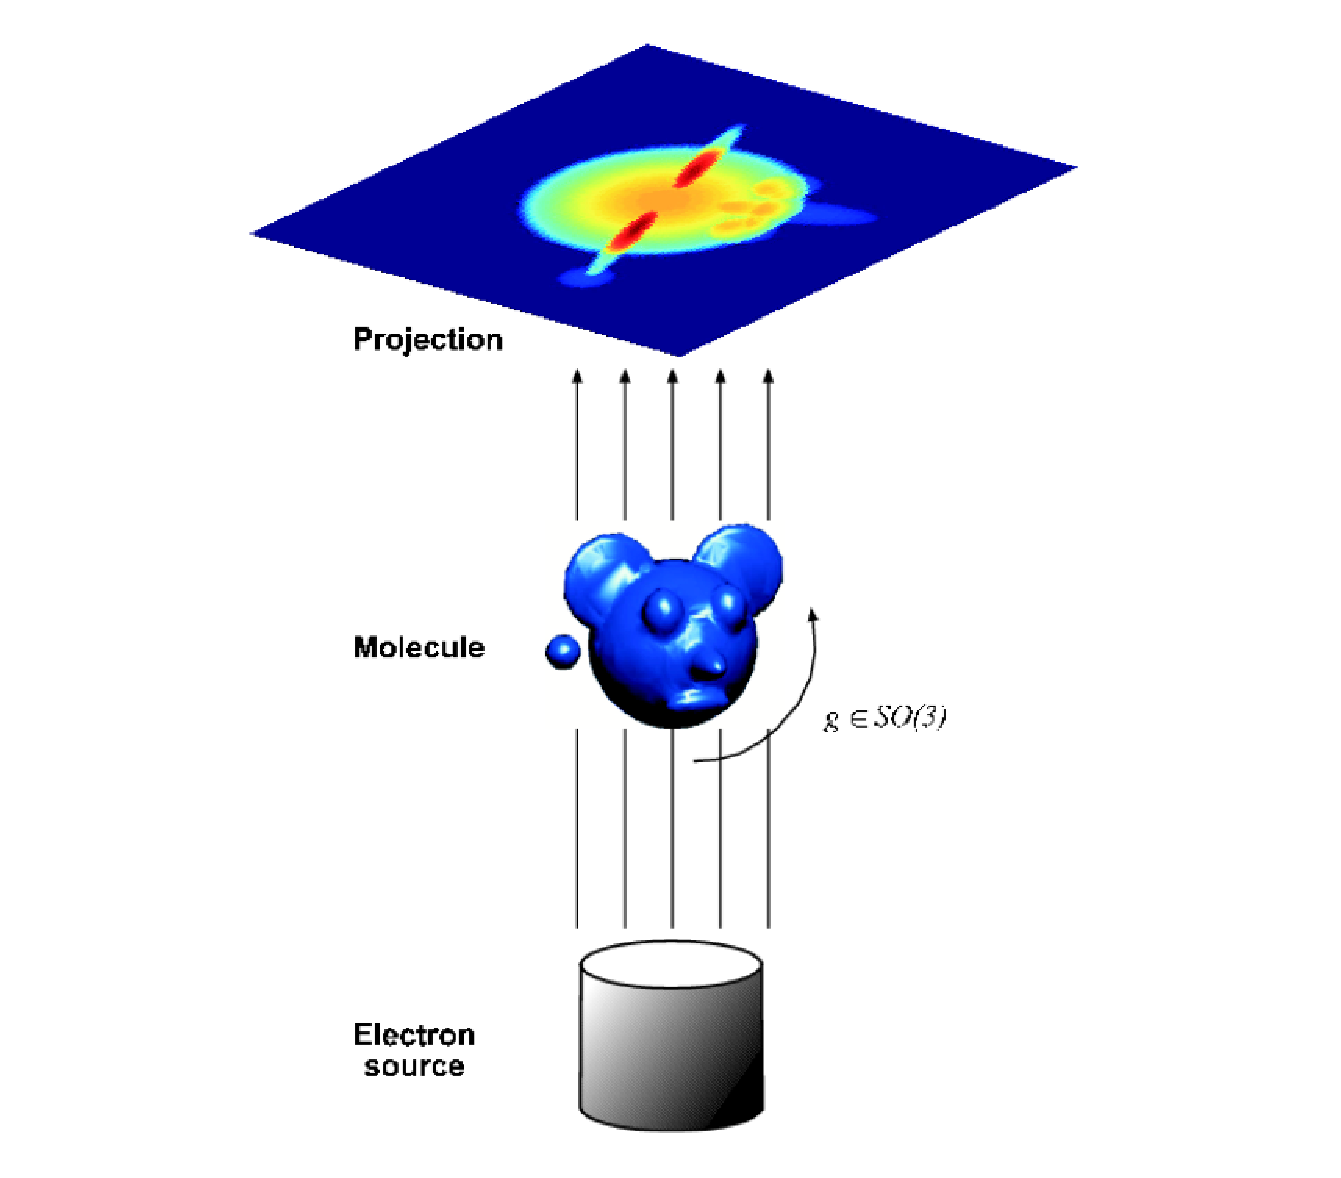
\includegraphics[width=0.9\textwidth]{figures/cryo-Singer.pdf} en local
            \framebox{\begin{minipage}{0.8\textwidth}\centering\vspace{1.5cm}\textcolor{DarkBeige}{\textbf{[ figures/cryo-Singer.pdf ]}}\\\small Schéma Cryo-EM / Projections\vspace{1.5cm}\end{minipage}}
        \end{column}
    \end{columns}
\end{frame}